\chapter{PENGUJIAN DAN EVALUASI}
	Pada bab ini akan dibahas uji coba dan evaluasi dari sistem yang dibuat. Sistem akan diuji coba fungsionalitasnya dengan menjalankan skenario pengujian performa pada web. Uji coba dilakukan untuk mengetahui kinerja sistem dengan lingkungan uji coba yang ditentukan.
	
	\section{Lingkungan Uji Coba}
		Lingkungan Uji coba sistem ini terdiri dari beberapa komponen yaitu \textit{web service dan task queue}, server basis data, server \textit{manager node}, dua server \textit{worker}. Server yang digunakan sistem menggunakan layanan \textit{Virtual Private Server} dari DigitalOcean, sedangkan \textit{web service} dan \textit{task queue} akan dibangun di komputer penulis. Spesifikasi untuk setiap komponen ditunjukkan pada Tabel \ref{tabelspesifikasi}.
		\begin{longtable}{|p{0.05\textwidth}|p{0.25\textwidth}|p{0.30\textwidth}|p{0.30\textwidth}|}
			\caption{Spesifikasi komponen} \label{tabelspesifikasi} \\
			\hline
			\textbf{No} & \textbf{Komponen} & \textbf{Perangkat Keras} & \textbf{Perangkat Lunak} \\ \hline
			\endhead
			\endfoot
			\endlastfoot
			1 & \textit{Web Service} \& \textit{Task Queue} & \textit{Processor} AMD FX-7600P Radeon R7, 4 Core, 8GB RAM, 250GB SSD & Ubuntu 18.04 LTS, Laravel 5.8, Python 3.6 \\ \hline
			2 & Basis Data & 1 Core Processor, 1GB RAM, 20GB SSD & Ubuntu 18.04 LTS, MySQL 5.7 \\ \hline
			3 & \textit{Manager Node} & 2 \textit{Core Processor}, 4GB RAM, 80GB SSD & Ubuntu 18.04 LTS, Python 3.6, Docker 18.09.6, Node.js 8.15, NPM 6.4.1, Chrome, Puppeteer 0.12.0, MySQL Client 5.7 \\ \hline
			4 & \textit{Worker} 1 & 2 \textit{Core Processor}, 4GB RAM, 80GB SSD & Ubuntu 18.04 LTS, Python 3.6, Docker 18.09.6, Node.js 8.15, NPM 6.4.1, Chrome, Puppeteer 0.12.0, MySQL Client 5.7 \\ \hline
			5 & \textit{Worker} 2 & 2 \textit{Core Processor}, 4GB RAM, 80GB SSD & Ubuntu 18.04 LTS, Python 3.6, Docker 18.09.6, Node.js 8.15, NPM 6.4.1, Chrome, Puppeteer 0.12.0, MySQL Client 5.7 \\ \hline
		\end{longtable}
	
		\indent Untuk akses ke setiap komponen, digunakan \textit{ip} publik yang disediakan untuk masing-masing komponen. Detail ditunjukkan pada Tabel \ref{ipserver}.
		\begin{longtable}{|p{0.05\textwidth}|p{0.25\textwidth}|p{0.30\textwidth}|p{0.30\textwidth}|}
			\caption{\textit{IP} dan \textit{hostname} server} \label{ipserver} \\
			\hline
			\textbf{No} & \textbf{Komponen} & \textbf{IP} & \textbf{Hostname} \\ \hline
			\endhead
			\endfoot
			\endlastfoot
			1 & \textit{Web Service} \& \textit{Task Queue} & 10.151.253.110 & night \\ \hline
			2 & Basis Data & 178.128.123.143 & NIGHT \\ \hline
			3 & \textit{Manager Node} & 167.71.194.235 & CLOUD \\ \hline
			4 & \textit{Worker Node} 1 & 165.22.55.82 & RAIN \\ \hline
			5 & \textit{Worker Node} 2 & 167.71.194.233 & STORM \\ \hline
		\end{longtable}
	
	\section{Skenario Uji Coba} \label{skenarioujicoba}
		Uji coba ini dilakukan untuk menguji apakah fungsionalitas yang diidentifikasikan terhadap kebutuhan sistem benar-benar telah diimplementasikan dan bekerja seperti yang seharusnya. Skenario pengujian dibedakan menjadi 2 bagian yaitu:
		\begin{itemize}
			\item \textbf{Uji Fungsionalitas} \\
				Pengujian yang dilakukan didasarkan pada fungsionalitas yang disajikan sistem.
			\item \textbf{Uji Performa} \\
				Pengujian ini dilakukan untuk mengetahui seberapa banyak \textit{load generator} yang bisa diatasi oleh sistem.
		\end{itemize} 
		
	\subsection{Skenario Uji Fungsionalitas}
		Uji fungsionalitas dibagi menjadi beberapa bagian antara lain yaitu \textit{user} mengelola skenario melalui web, \textit{user} mengirim request uji beban melalui web, penggunaan \textit{task queue} terhadap \textit{request user}, pengambil data uji beban, \textit{user} melihat hasil uji beban melalui web.
		
		\subsubsection{Uji Fungsionalitas \textit{User} Mengelola Skenario}
			Uji coba ini dilakukan dengan mengakses sistem melalui rute \texttt{/skenario}. Pengguna akan mengirimkan \textit{http request} kepada \textit{web service} yang telah disediakan. Rancangan pengujian dan hasil yang diharapkan ditunjukkan pada Tabel \ref{tabelujiskenario}.
			\begin{longtable}{|p{0.05\textwidth}|p{0.25\textwidth}|p{0.30\textwidth}|p{0.30\textwidth}|}
				\caption{Skenario uji fungsionalitas \textit{user} mengelola skenario} \label{tabelujiskenario} \\ \hline
				\textbf{No} & \textbf{Rute} & \textbf{Uji Coba} & \textbf{Hasil \& Harapan} \\ \hline
				\endhead
				\endfoot
				\endlastfoot
				1 & /skenario & Mengirimkan \textit{request} menuju rute \textit{web service} melalui \textit{browser} & \textit{Request} berhasil diterima oleh \textit{web service}, kemudian \textit{web service} mengirimkan umpan balik berupa data skenario dari pengguna yang ditampilkan di \textit{browser} \\ \hline
				2 & /skenario/create & Mengirimkan \textit{request} menuju rute \textit{web service} melalui \textit{browser} & \textit{Request} berhasil diterima oleh \textit{web service} dan halaman untuk membuat skenario ditampilkan di \textit{browser} \\ \hline
				3 & /skenario & Mengirimkan \textit{request} pembuatan skenario menuju rute \textit{web service} melalui \textit{browser} menggunakan metode \textit{POST} & \textit{Web service} berhasil menyimpan data skenario di basis data dan di setiap \textit{node host} dalam bentuk file konfig \\ \hline
				4 & /skenario/\{id\} & Mengirimkan \textit{request} untuk menghapus skenario menuju rute \textit{web service} melalui \textit{browser} menggunakan metode \textit{POST} & \textit{Web service} berhasil menghapus data skenario di basis data dan di setiap \textit{node host} \\ \hline
			\end{longtable}
		
		\subsubsection{Uji Fungsionalitas \textit{User} Mengirim Request Uji Beban}
			Uji coba ini dilakukan dengan mengakses sistem melalui rute \texttt{/worker}. Pengguna akan mengirimkan \textit{http request} kepada \textit{web service} yang telah disediakan. Rancangan pengujian dan hasil yang diharapkan ditunjukkan pada Tabel \ref{tabelujirequest}.
			\begin{longtable}{|p{0.05\textwidth}|p{0.25\textwidth}|p{0.30\textwidth}|p{0.30\textwidth}|}
				\caption{Skenario uji fungsionalitas \textit{user} mengirim request uji beban} \label{tabelujirequest} \\ \hline
				\textbf{No} & \textbf{Rute} & \textbf{Uji Coba} & \textbf{Hasil \& Harapan} \\ \hline
				\endhead
				\endfoot
				\endlastfoot
				1 & /worker & Mengirimkan \textit{request} menuju rute \textit{web service} melalui \textit{browser} & \textit{Request} berhasil diterima oleh \textit{web service}, kemudian \textit{web service} menampilkan halaman untuk mengatur jumlah \textit{worker(load generator)} di \textit{browser} \\ \hline
				2 & /worker & Mengirimkan \textit{request} menuju rute \textit{web service} melalui \textit{browser} menggunakan metode \textit{POST} & \textit{Web service} berhasil menyimpan data \textit{worker} dan membuat antrian \textit{request} di dalam basis data  \\ \hline
			\end{longtable}
		
		\subsubsection{Uji Fungsionalitas Penggunaan \textit{Task Queue} Terhadap \textit{Request User}}
			\begin{figure}[H]
				\centering
				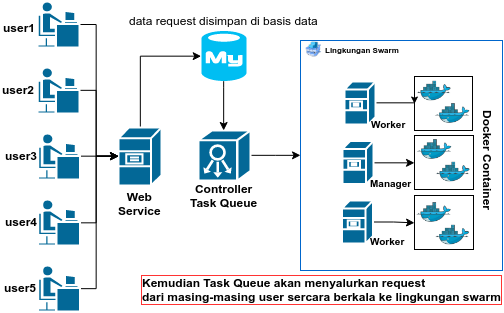
\includegraphics[width=10cm,height=7cm]{Images/C-5/taskqueue.png}
				\caption{Struktur diagram \textit{Puppeteer}}
				\label{gambartaskqueue}
			\end{figure}
			Uji coba ini dilakukan dengan cara menjalankan \textit{script} yang menggunakan bahasa pemrograman \textit{Python} pada \textit{crontab} yang ada di \textit{linux} dan dijadwalkan setiap 1 menit. Setiap kali pengguna mengirim \textit{request} uji beban melalui web, akan disimpan di basis data \textit{MySQL}. Ketika ada daftar antrian yang ada di basis data \textit{MySQL}, \textit{script} akan mengeksekusi hanya satu \textit{request} yang memiliki \textit{timestamp} paling awal dari beberapa \textit{request} yang lain dan akan dilakukan pengujian terhadap skenario yang dikirim. Setelah pengujian skenario selesai, status akan diubah menjadi \textit{done} dan \textit{script} akan mengeksekusi \textit{request} yang lain satu-persatu. Pada pengujian ini akan dilakukan oleh 5 pengguna yang akan melakukan \textit{request} uji beban. Gambaran pengujian ditunjukkan pada Gambar \ref{gambartaskqueue}.
			
		
		\subsubsection{Uji Fungsionalitas Pengambil Data Uji Beban}
			Uji coba ini dilakukan dengan cara menjalankan \textit{script puppeteer} pada setiap kontainer. \textit{script puppeteer} akan dijalankan ketika ada \textit{request} dari pengguna melalui \textit{web service} yang disediakan sistem. Gambaran pengujian ditunjukkan pada Gambar \ref{ambilhasiluji}.
			\begin{figure}[H]
				\centering
				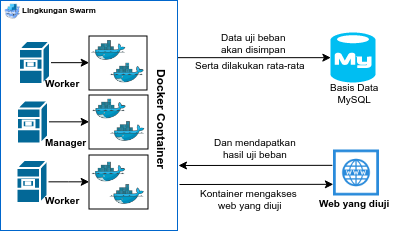
\includegraphics[width=9cm,height=6cm]{Images/C-5/ambilhasiluji.png}
				\caption{Struktur diagram \textit{Puppeteer}}
				\label{ambilhasiluji}
			\end{figure}
		
		\subsubsection{Uji Fungsionalitas \textit{User} Melihat Hasil Uji Beban}
			Uji coba ini dilakukan dengan mengakses sistem melalui rute \texttt{/hasil}. Pengguna akan mengirimkan \textit{http request} kepada \textit{web service} yang telah disediakan. Rancangan pengujian dan hasil yang diharapkan ditunjukkan pada Tabel \ref{tabelujihasil}.
			\begin{longtable}{|p{0.05\textwidth}|p{0.25\textwidth}|p{0.30\textwidth}|p{0.30\textwidth}|}
				\caption{Skenario uji fungsionalitas \textit{user} melihat hasil uji beban} \label{tabelujihasil} \\ \hline
				\textbf{No} & \textbf{Rute} & \textbf{Uji Coba} & \textbf{Hasil \& Harapan} \\ \hline
				\endhead
				\endfoot
				\endlastfoot
				1 & /hasil/rata-rata & Mengirimkan \textit{request} menuju rute \textit{web service} melalui \textit{browser} & \textit{Request} berhasil diterima oleh \textit{web service}, kemudian \textit{web service} menampilkan hasil perhitungan rata-rata untuk hasil uji beban \\ \hline
				2 & /hasil/error-console & Mengirimkan \textit{request} menuju rute \textit{web service} melalui \textit{browser} & \textit{Request} berhasil diterima oleh \textit{web service}, kemudian \textit{web service} menampilkan daftar \textit{error console} yang terekam pada \textit{browser} \\ \hline
				3 & /hasil/images & Mengirimkan \textit{request} menuju rute \textit{web service} melalui \textit{browser} & \textit{Request} berhasil diterima oleh \textit{web service}, kemudian \textit{web service} menampilkan hasil tangkapan layar web yang diuji pada \textit{browser} \\ \hline
			\end{longtable}
		
	\subsection{Skenario Uji Performa}
		Sistem \textit{load generator} dan pengambil data uji beban dibangun pada 3 buah \textit{node host} yang terpasang di lingkungan \textit{swarm}.  Sebelum dilakukan uji performa, dilakukan pemasangan \textit{load generator} yang diinisiasi pada terminal \textit{manager node}, kemudian \textit{manager node} akan mendistribusikan kontainer ke setiap \textit{node host} yang tergabung. Setelah selesai, data dari setiap kontainer akan disimpan di basis data. Uji coba akan dilakukan secara bertahap untuk membuat 100, 200, 300, 400 dan 500 kontainer, status awal kontainer sebelum diberikan \textit{request} akan \textit{sleep}. Setelah itu uji coba performa dilakukan untuk menguji performa sistem terhadap jumlah \textit{load generator} yang dikirimkan oleh pengguna. Pengujian akan dikirimkan oleh pengguna melalui \textit{web service} yang disediakan sistem. Jumlah \textit{load generator} yang akan diuji mulai dari 100, 200, 300, 400 dan 500. Hasil yang diharapkan dari pengujian performa sistem yaitu \textit{CPU Usage}, \textit{Memory} dan \textit{Disk Usage} yang digunakan pada setiap \textit{node host}.
	
	\section{Hasil Uji Coba dan Evaluasi}
		Berikut dijelaskan hasil uji coba dan evaluasi berdasarkan skenario yang sudah dijelaskan pada bab \ref{skenarioujicoba}.
		
		\subsection{Uji Fungsionalitas}
			Berikut dijelaskan hasil pengujian fungsionalitas pada sistem yang sudah dibangun.
			
			\subsubsection{Uji Fungsionalitas \textit{User} Mengelola Skenario}
				Uji coba ini dilakukan dengan mengakses sistem melalui rute yang telah ditentukan pada Tabel \ref{tabelujiskenario}. Pengguna akan mengirim http request kepada web service yang telah
				disediakan. Hasil uji coba seperti tertera pada Tabel \ref{tabelhasilujiskenario}.
				\begin{longtable}{|p{0.05\textwidth}|p{0.25\textwidth}|p{0.30\textwidth}|p{0.30\textwidth}|}
					\caption{Skenario uji fungsionalitas \textit{user} mengelola skenario} \label{tabelhasilujiskenario} \\ \hline
					\textbf{No} & \textbf{Rute} & \textbf{Uji Coba} & \textbf{Hasil \& Harapan} \\ \hline
					\endhead
					\endfoot
					\endlastfoot
					1 & /skenario & Mengirimkan \textit{request} menuju rute \textit{web service} melalui \textit{browser} & Berhasil \\ \hline
					2 & /skenario/create & Mengirimkan \textit{request} menuju rute \textit{web service} melalui \textit{browser} & Berhasil \\ \hline
					3 & /skenario & Mengirimkan \textit{request} pembuatan skenario menuju rute \textit{web service} melalui \textit{browser} menggunakan metode \textit{POST} & Berhasil \\ \hline
					4 & /skenario/\{id\} & Mengirimkan \textit{request} untuk menghapus skenario menuju rute \textit{web service} melalui \textit{browser} menggunakan metode \textit{POST} & Berhasil \\ \hline
				\end{longtable}
				
			\subsubsection{Uji Fungsionalitas \textit{User} Mengirim Request Uji Beban}
				Uji coba ini dilakukan dengan mengakses sistem melalui rute yang telah ditentukan pada Tabel \ref{tabelujirequest}. Pengguna akan mengirim http request kepada web service yang telah
				disediakan. Hasil uji coba seperti tertera pada Tabel \ref{tabelhasilujirequest}.
				\begin{longtable}{|p{0.05\textwidth}|p{0.25\textwidth}|p{0.30\textwidth}|p{0.30\textwidth}|}
					\caption{Skenario uji fungsionalitas \textit{user} mengirim request uji beban} \label{tabelhasilujirequest} \\ \hline
					\textbf{No} & \textbf{Rute} & \textbf{Uji Coba} & \textbf{Hasil \& Harapan} \\ \hline
					\endhead
					\endfoot
					\endlastfoot
					1 & /worker & Mengirimkan \textit{request} menuju rute \textit{web service} melalui \textit{browser} & Berhasil \\ \hline
					2 & /worker & Mengirimkan \textit{request} menuju rute \textit{web service} melalui \textit{browser} menggunakan metode \textit{POST} & Berhasil \\ \hline
				\end{longtable}
				
			\subsubsection{Uji Fungsionalitas Penggunaan \textit{Task Queue} Terhadap \textit{Request User}}
				
			\subsubsection{Uji Fungsionalitas Pengambil Data Uji Beban}
				
			\subsubsection{Uji Fungsionalitas \textit{User} Melihat Hasil Uji Beban}
				Uji coba ini dilakukan dengan mengakses sistem melalui rute yang telah ditentukan pada Tabel \ref{tabelujihasil}. Pengguna akan mengirim http request kepada web service yang telah
				disediakan. Hasil uji coba seperti tertera pada Tabel \ref{tabelhasilujihasil}.
				\begin{longtable}{|p{0.05\textwidth}|p{0.25\textwidth}|p{0.30\textwidth}|p{0.30\textwidth}|}
					\caption{Skenario uji fungsionalitas \textit{user} melihat hasil uji beban} \label{tabelhasilujihasil} \\ \hline
					\textbf{No} & \textbf{Rute} & \textbf{Uji Coba} & \textbf{Hasil \& Harapan} \\ \hline
					\endhead
					\endfoot
					\endlastfoot
					1 & /hasil/rata-rata & Mengirimkan \textit{request} menuju rute \textit{web service} melalui \textit{browser} & Berhasil \\ \hline
					2 & /hasil/error-console & Mengirimkan \textit{request} menuju rute \textit{web service} melalui \textit{browser} & Berhasil \\ \hline
					3 & /hasil/images & Mengirimkan \textit{request} menuju rute \textit{web service} melalui \textit{browser} & Berhasil \\ \hline
				\end{longtable}
				

		\subsection{Uji Performa}